\chapter{Carla Umgebung}
\label{sec:carla umgebung}

\section{Aufbau Testszenario in Carla}

Um den Eye Tracker in Zusammenhang mit Carla testen zu können, muss eine Testumgebung in Carla angelegt werden. In Abbildung \ref{fig:code_structure_carla_1} sind die groben Schritte zur Erzeugung einer Testumgebung zu erkennen. Hier ist das Zusammenspiel zwischen dem Carla Server und dem Carla Client besonders hervorgehoben. Der Host-PC ist in diesem Fall der Computer, auf welchem der Fahrsimulator ausgeführt wird. Auf diesem ist Windows als Betriebssystem installiert. Im gesamten Zeitraum der Projektarbeit wird der Carla Server immer lokal auf diesem Computer laufen. Der Carla Server ist für die eigentliche Simulation sowie der Aktoren in ihr verantwortlich. Der Client läuft auf demselben Computer und kann Anfragen an den Server senden. Auf diese Weise kann der Client die Simulation aktiv beeinflussen oder Daten wie bspw. Positionsdaten oder Bilddaten vom Server anfragen. \cite{lit_website_carla_documentation}

Der Carla Server kann heruntergeladen werden und direkt als ausführbares Programm gestartet werden. Anders als der Carla Client, welcher selbst in Python geschrieben werden muss. Dafür kann dieser auch nach den eigenen Anforderungen individuell aufgesetzt werden. In der Dokumentation von Carla gibt es einige Beispiele wie ein Client aufgebaut werden kann, nach welchen sich der Client für diese Projektarbeit auch orientiert \cite{lit_code_api}. Zur Serververbindung nutzt er das Application Programming Interface (\acrshort{api}) des Carla Servers. Der Client wurde so geschrieben, dass er zuerst versucht, eine Verbindung zum Carla Server aufzubauen. Anschließend holt er sich wichtige Informationen über die simulierte Welt und mögliche \gls{Spawnpunkt}e für bspw. Fahrzeuge vom Server. Unter Actors werden in diesem Kontext unter anderem Fahrzeuge und Sensoren bezeichnet. Der Client fordert eine Liste aller in der aktuell simulierten Welt vorhandenen Fahrzeuge und Sensoren an und "zerstört" diese anschließend. Somit wird sichergestellt, dass keine Aktoren aus einer vorherigen Sitzung in die neue Sitzung mitgebracht werden. Nachdem die simulierte Welt wieder einen fest definierten Ausgangszustand angenommen hat, beginnt der Client damit, einen Mercedes Sprinter zu spawnen. Abbildung \ref{fig:code_structure_carla_2} stellt die Fortsetzung des Prozesses dar. Nachdem das Fahrzeug vom Server in der Welt erzeugt wurde, fordert der Client die Erzeugung von zwei Sensoren an. Beide Sensoren sollen an das erzeugte Fahrzeug geknüpft sein. Der erste Sensor soll den Rot-Grün-Blau (\acrshort{rgb})Farbraum erfassen. Der zweite Sensor soll die Instance Segmentation erfassen. Auf diese und die Verarbeitung der daraus resultierenden Daten wird weiter unten genauer eingegangen. 

\begin{figure}[h!]
	\begin{center}
		
\includegraphics[scale=0.1]{code_structure_carla_1}
		\caption{Visuelle Darstellung des Codes zur Carla Testumgebung Teil 1/2, Quelle: \cite{lit_software_eraserio},\cite{lit_website_carla_documentation}} \label{fig:code_structure_carla_1}
	\end{center}
\end{figure}

\begin{figure}[h!]
	\begin{center}
		
\includegraphics[scale=0.1]{code_structure_carla_2}
		\caption{Visuelle Darstellung des Codes zur Carla Testumgebung Teil 2/2, Quelle: \cite{lit_software_eraserio},\cite{lit_website_carla_documentation}} \label{fig:code_structure_carla_2}
	\end{center}
\end{figure}

\section{Sensor Auswertung}

\subsection{Verschiedene Sensortypen}
Der \acrshort{rgb}-Sensor liefert ein Bild an den Client, welches einer Kameraaufnahme gleicht. Durch die roten, grünen und blauen Farbanteile kann ein Bild erzeugt werden, welches für die Testperson im Fahrsimulator die simulierte Welt in Farbe darstellt. Die simulierte Welt kann durch diesen \acrshort{rgb}-Sensor wie durch eine Kameralinse betrachtet werden. Der Server berechnet die Welt in Zahlen und der Sensor ermöglicht es der Testperson im Fahrsimulator diese auf zahlen basierende Welt visuell wahrzunehmen. Die Objekte und die Farben der Welt werden so dargestellt, wie sie für den Menschen natürlich sind. Ein Baum hat die Form eines Baums und besitzt grüne Blätter und einen braunen Stamm. In Carla kann bei Bedarf auch ein Lidar-Sensor platziert werden. Dieser erzeugt ebenfalls ein Bild der simulierten Umgebung. Dieses würde den Baum dann aber als eine Art Punktwolke in einer schwarzen Umgebung darstellen. Ein Lidar-Sensor würde die Welt in einer anderen Art und Weise wahrnehmen, wodurch auch ein anderes Bild im Vergleich zu einem \acrshort{rgb}-Sensor entstehen würde. 

\subsection{Instance Segmentation Sensor}
Der Instance Segmentation Sensor ist in seiner Funktion etwas spezieller. Dieser kategorisiert die Objekte in der Welt in Gruppen ein und weißt ihnen IDs zu. Er färbt gewisse Objektgruppen nach ihrer jeweiligen Gruppenzugehörigkeit. Bspw. werden Straßen hellgrün und Gebäude dunkelblau gezeichnet. Zusätzlich besitzt jedes Objekt eine eindeutige Identifikationsnummer (\acrshort{id}). So hat jedes Fahrzeug in der simulierten Welt eine eindeutige, ihm zugewiesene \acrshort{id}. Damit sowohl die Gruppenzugehörigkeit, als auch die \acrshort{id} in die Bildinformation der Sensorausgabe übergeben werden können, gibt es zwei Codierungsmechanismen. Bei der Sensorausgabe handelt es sich wie beim \acrshort{rgb}-Sensor um eine Farbbildausgabe bestehend aus rot-, grün- und blau-Anteilen. Die Zugehörigkeit eines Objekts in eine bestimmte Gruppe wird durch den Rot-Anteil des Bildes an der Stelle des Objektes bestimmt. Die Tabelle \ref{tab:rot_tag} stellt die korrekte Zuweisung zwischen dem Rot-Wert und der jeweiligen Eingruppierung dar. Im Code wurde sich auf diese Zuweisung gestützt. Es muss berücksichtigt werden, dass bei unterschiedlichen Versionen von Carla eine unterschiedliche Zuweisung erfolgt \cite{lit_website_carla_documentation}. 


\begin{table}[h]
	\begin{center}
		{\small %
			\begin{tabular}{c l}
				\toprule
				\textbf{Rot-Wert} & \textbf{Gruppe} \\
				\midrule
				0  & Unlabeled \\
				1  & Roads \\
				2  & SideWalks \\
				3  & Building \\
				4  & Wall \\
				5  & Fence \\
				6  & Pole \\
				7  & TrafficLight \\
				8  & TrafficSign \\
				9  & Vegetation \\
				10 & Terrain \\
				11 & Sky \\
				12 & Pedestrian \\
				13 & Rider \\
				14 & Car \\
				15 & Truck \\
				16 & Bus \\
				17 & Train \\
				18 & Motorcycle \\
				19 & Bicycle \\
				20 & Static \\
				21 & Dynamic \\
				22 & Other \\
				23 & Water \\
				24 & RoadLine \\
				25 & Ground \\
				26 & Bridge \\
				27 & RailTrack \\
				28 & GuardRail \\
				\bottomrule
			\end{tabular}
		}%
	\end{center}
	\caption{Zuweisung Rot-Wert und Objektgruppe bei Carla Version 0.9.15, Quelle: \cite{lit_website_carla_documentation}}\label{tab:rot_tag}
	
\end{table}



Die \acrshort{id} wird in den grün- und blau-Anteil des Bildes codiert. Liegt bspw. ein grün-Anteil von 22 und ein blau-Anteil von 232 vor, dann lautet die \acrshort{id} des Objektes "22-232".

Der Client fordert die Sensorausgabe des Instance Segmentation Sensors in regelmäßigen Abständen vom Server an. Anschließend extrahiert er die \acrshort{rgb}-Werte und wertet diese nach den oben beschriebenen Zuordnungen aus. Die Auswertung erfolgt dabei immer genau an einem Pixel. Die Position des Pixels ist definiert durch die aktuelle Ausgabe der geschätzten Blickposition vom Eye Tracker. 

\subsection{Optimierung der Performance}
Der Rechenaufwand, den der Server leisten muss, um die Sensorausgabe zu generieren, ist nicht zu vernachlässigen. Bei der \acrshort{rgb}-Ausgabe sind nicht viele Abstriche möglich, da die Testperson ein Bild von hoher Auflösung für die große Leinwand im Fahrsimulator benötigt. Die Sensorausgabe des Instance Segmentation Sensors kann hingegen auch mit einer geringeren Auflösung generiert werden. Dadurch wird Rechenleistung gespart und da die Sensorausgabe nur im Hintergrund benötigt wird, macht es für die Testperson auch keinen bemerkbaren Unterschied. 

Damit das Zusammenspiel zwischen Eye Tracker und Sensor allerdings weiterhin funktioniert, müssen die Werte des Eye Trackers ebenfalls auf die herunterskalierte Sensorausgabe umgerechnet werden. In Abbildung \ref{fig:scale} ist diese Skalierung grafisch dargestellt. Durch den Faktor zehn werden aus den Originalbilddaten jeweils 10x10 Pixel auf ein einzelnes Pixel herunterskaliert. Alle Pixel innerhalb dieses 10x10 Rasters, wie bspw. das Pixel bei Position x=7 und y=4 werden dann auf ein Pixel bezogen. Dadurch wird offensichtlich die Genauigkeit verringert, da der Eye Tracker zwar Tracking Daten bezogen auf die Originalauflösung ausgibt, dann aber auf die herunterskalierte Instance Segmentation Sensorausgabe beziehen muss. Bei einer Reduzierung der Auflösung um Faktor zehn wurden allerdings keine bemerkbaren, negativen Einflüsse auf die Funktion des Eye Trackers festgestellt.



\begin{figure}[h]
	\begin{center}
		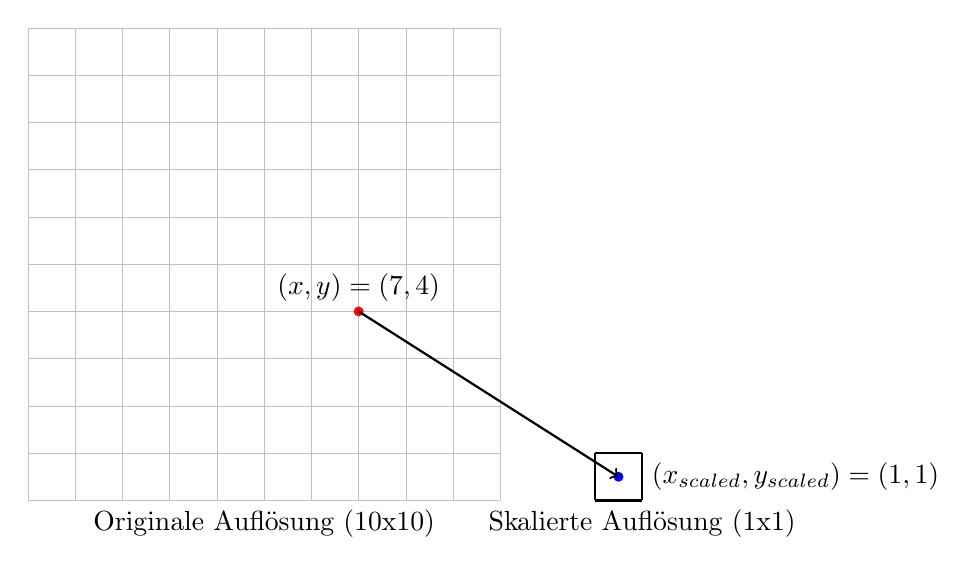
\begin{tikzpicture}[scale=0.6]
			% Großes Raster (Originale Auflösung)
			\draw[step=1cm, gray!50, very thin] (0,0) grid (10,10);
			\node at (5,-0.5) {Originale Auflösung (10x10)};
			
			% Kleines Raster (herunterskalierte Auflösung)
			
			\draw[step=1cm, black, thick] (12,0) grid (13,1);
			\node at (13,-0.5) {Skalierte Auflösung (1x1)};
			
			% Punkt in der großen Skala
			\fill[red] (7, 4) circle (3pt);
			\node[above] at (7, 4) {$(x,y) = (7,4)$};
			
			% Skalierter Punkt
			\fill[blue] (12.5,0.5) circle (3pt);
			\node[right] at (13,0.5) {$(x_{scaled}, y_{scaled}) = (1,1)$};
			
			% Pfeil zur Transformation
			\draw[->, thick] (7,4) -- (12.5,0.5);
			
		\end{tikzpicture}
		\caption{Herunterskalierung der Eye-Tracking-Daten um Faktor 10}\label{fig:scale}
	\end{center}
	
\end{figure}


\section{Darstellung der Daten in Carla}
Die Daten des Eye Trackers werden nicht direkt in Carla dargestellt, sondern in einem transparenten Windows Fenster, welches über die Carla Client Anwendung geschoben wird. Die Inhalte dieses transparenten Fensters können allerdings in Zukunft bei Bedarf in die Carla Anwendung selbst implementiert werden.

In Abbildung \ref{fig:carla_hud} ist die graphische Darstellung der Daten des Eye Trackers im transparenten Fenster zu erkennen. Das erste Anzeigeelement ist der lila gefärbte Kreis. Dieser zeigt die geschätzte Blickposition des Eye Trackers an. Bei den Werten handelt es sich um die Rohdaten, welche noch nicht durch unsere Korrekturfunktion bearbeitet wurden. Als zweites wird hier der rote Punkt angezeigt. In der Realität ist das der Mauszeiger. Zur besseren Sichtbarkeit wurde dieser durch einen roten Kreis hervorgehoben. Der Mauszeiger wurde dazu verwendet, um die Performance des Eye Trackers messbar zu machen. Die Testperson hat den Mauszeiger bewegt und auf diesen geschaut. Dadurch war der Wert der tatsächlichen Blickposition bekannt und konnte mit dem Wert für die geschätzte Blickposition verglichen werden. Während der normalen Verwendung des Eye Trackers spielt dieser aber keine Rolle. Als drittes Element wird der schwarze Punkt angezeigt. Dieser liefert genauso wie der lila farbene Kreis die geschätzte Blickposition auf der Leinwand. Allerdings werden für die Darstellung des schwarzen Punktes die von uns korrigierten Werte verwendet. Der schwarze Punkt ist dementsprechend der eigentlich geltende Wert. Das vierte Anzeigeelement ist die textbasierte Ausgabe. In dieser werden verschiedene Werte ausgegeben, welche gleich noch detaillierter beschrieben werden. Das kleine türkisfarbene Fenster oben links ist die Ausgabe des Instance Segmentation Sensors. Diese kann bei der Verwendung des Eye Trackers im Hintergrund laufen und muss nicht weiter beachtet werden.




\begin{figure}[h!]
	\begin{center}
		
\includegraphics[scale=0.35]{carla_hud}
		\caption{Darstellung der Daten in Carla, Quelle: \cite{lit_software_carla}, \cite{lit_software_canva}} \label{fig:carla_hud}
	\end{center}
\end{figure}


In Abbildung \ref{fig:carla_hud_2} sind die textbasierten Daten aus Anzeigeelement vier in Abbildung \ref{fig:carla_hud} nochmals genauer dargestellt. Es werden Informationen über den Verbindungsstatus des Eye Trackers, die aktuell geschätzten Blickkoordinaten, die grobe Blickrichtung und die Instance Segmentation Auswertung gegeben. Die 'Looking Direction' gibt dabei die grobe Blickrichtung der Testperson an. Der 'Tag' ist die Einordnung des Objektes auf welches die Testperson schaut in eine Objektgruppe und die 'Instance ID' die eindeutige Identifikationsnummer für selbiges Objekt. Der grüne Punkt unten gibt die aktuelle Tracking Confidence des Eye Trackers nochmals in Form einer Ampel aus. Dadurch kann sofort erkannt werden, wenn der Eye Tracker die Testperson nicht mehr korrekt erfasst.  

\begin{figure}[h!]
	\begin{center}
		
\includegraphics[scale=1]{carla_hud_2}
		\caption{Darstellung der textbasierten Daten in Carla, Quelle: \cite{lit_software_carla}, \cite{lit_software_canva}} \label{fig:carla_hud_2}
	\end{center}
\end{figure}
